\documentclass{beamer}
\usepackage{graphicx}
\usepackage{hyperref}



\title{Online Outlier Exploration over Large Datasets}
\author{Matthias Hansen \\
        \texttt{matthias.hansen@rwth-aachen.de}}
\date{Data Mining and Multimedia Search}
\institute{RWTH Aachen University}
\begin{document}
\frame{\titlepage}
\section{Outlier Detection}



\begin{frame}{Example: Gaussian Distribution $\mathcal{N}(0,1)$}
    \centering
    \includegraphics<1>[width=.7\textwidth]{images/gaussian.png}
    \includegraphics<2>[width=.7\textwidth]{images/gaussian_lines.png}

    \visible<2>{Within \alert{red} lines $\implies$ inlier.

    Outside \alert{red} lines $\implies$ outlier.}
\end{frame}

\begin{frame}{The Traditional Approach: Statistical Distributions}
    \begin{itemize}
        \item Statistical Distribution of Data must be known.
        \item Can sometimes be Inferred (e.g. using Expectation Maximization).
        \item Linear Runtime.
    \end{itemize}
\end{frame}

\begin{frame}{Counterexample: Geospatial Data}
    \begin{itemize}
        \item OpenStreetMap Data for South America and South Pacific Islands

        \item Roughly 1.3 Gigabytes of Data. (Raw Positions)

        \item Obtained from \texttt{http://download.geofabrik.com}
    \end{itemize}
    \begin{center}
    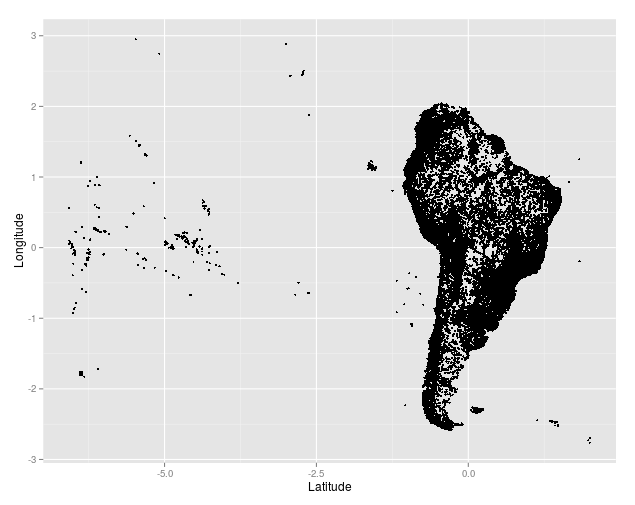
\includegraphics[width=.7\textwidth]{images/south_america.png} 
    \end{center}
\end{frame}

\begin{frame}
    \begin{center}
    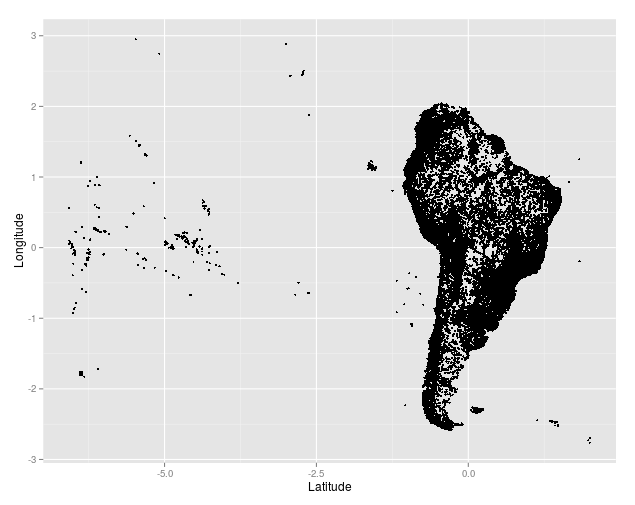
\includegraphics[width=.7\textwidth]{images/south_america.png} 
    \end{center}
    \begin{itemize}
        \item Task: Find Wrong Data Inserted by Malicious Users.

        \item Example: Someone placed a Shop in the middle of the ocean.

    \end{itemize}
\end{frame}

\begin{frame}{Distance-Based Outliers}
    \begin{block}{Distance-Based Outliers}
        Let DB be a sequence of vectors, dist a distance function.

        A point $p\in DB$ is a distance based outlier w.r.t. parameters $k$ and $\varepsilon$
        iff. $|\{q\in DB | dist(p,q) < \varepsilon\}| < k$
    \end{block}

    \begin{itemize}
        \item Same notion as ``non-core points'' in DBSCAN.
        \item Meaningful for geospatial data with Euclidean Distance.
    \end{itemize}
    %TODO add explanatory graphic here
\end{frame}


\begin{frame}{Performance Considerations}
    \begin{itemize}
        \item Similarly to DBSCAN, naive computation in $\mathcal{O}(n^2)$ 
        \item But: $\mathcal{O}(n\log(n))$ computation possible using spatial index structure ($k$-dimensional trees)
        \item Cao reports a Runtime in the Order of Magnitude of 2 hours using (apparently) an $n\log(n)$ algorithm implemented in Java.
        \item My Experiments: one Run of the $\mathcal{O}(n\log(n)$ Algorithm Takes Roughly 10 Minutes Using Mount and Arya's Optimized NN Library (written in C++).
            %TODO: add citations here.
        \item Due to (slightly) Above Linear Runtime, Datasets that are in the order of Magnitude of 10 or even 100GB are going to take quite long, even on fast machines and with optimized implementations.
            
    \end{itemize}
\end{frame}

\end{document}
